


\tikzset{every picture/.style={line width=0.75pt}} %set default line width to 0.75pt        

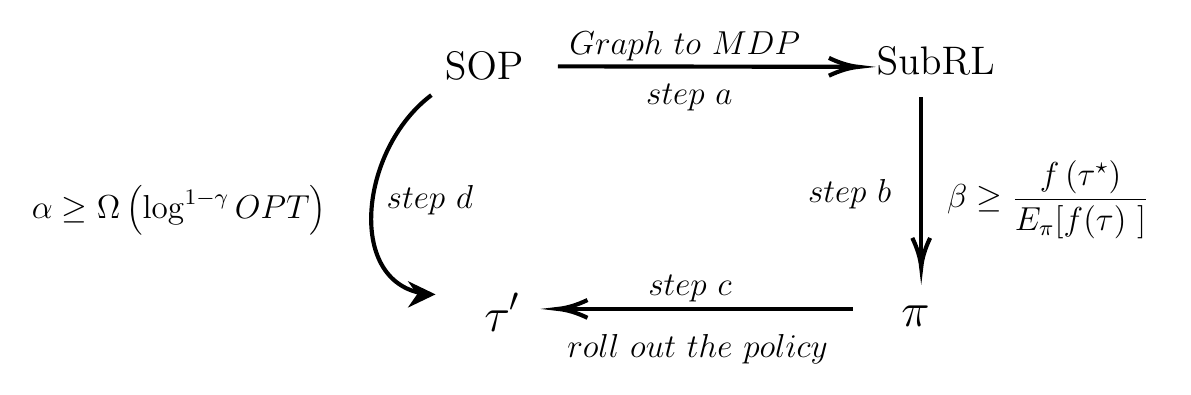
\begin{tikzpicture}[x=0.75pt,y=0.75pt,yscale=-1,xscale=1]
%uncomment if require: \path (0,621); %set diagram left start at 0, and has height of 621

%Straight Lines [id:da044623699124812344] 
\draw [line width=1.5]    (780,84.13) -- (921.75,84.37) ;
\draw [shift={(924.75,84.38)}, rotate = 180.1] [color={rgb, 255:red, 0; green, 0; blue, 0 }  ][line width=1.5]    (14.21,-4.28) .. controls (9.04,-1.82) and (4.3,-0.39) .. (0,0) .. controls (4.3,0.39) and (9.04,1.82) .. (14.21,4.28)   ;
%Straight Lines [id:da06082320338508107] 
\draw [line width=1.5]    (922,201) -- (783,201) ;
\draw [shift={(780,201)}, rotate = 360] [color={rgb, 255:red, 0; green, 0; blue, 0 }  ][line width=1.5]    (14.21,-4.28) .. controls (9.04,-1.82) and (4.3,-0.39) .. (0,0) .. controls (4.3,0.39) and (9.04,1.82) .. (14.21,4.28)   ;
%Straight Lines [id:da2814232469339797] 
\draw [line width=1.5]    (955,99.13) -- (955,178) ;
\draw [shift={(955,181)}, rotate = 270] [color={rgb, 255:red, 0; green, 0; blue, 0 }  ][line width=1.5]    (14.21,-4.28) .. controls (9.04,-1.82) and (4.3,-0.39) .. (0,0) .. controls (4.3,0.39) and (9.04,1.82) .. (14.21,4.28)   ;
%Curve Lines [id:da05840412220817237] 
\draw [line width=1.5]    (719,98) .. controls (684.08,124.19) and (677.39,189.9) .. (717.17,193.82) ;
\draw [shift={(721,194)}, rotate = 180] [fill={rgb, 255:red, 0; green, 0; blue, 0 }  ][line width=0.08]  [draw opacity=0] (13.4,-6.43) -- (0,0) -- (13.4,6.44) -- (8.9,0) -- cycle    ;

% Text Node
\draw (724,76) node [anchor=north west][inner sep=0.75pt]  [font=\Large] [align=left] {SOP};
% Text Node
\draw (932,73) node [anchor=north west][inner sep=0.75pt]  [font=\Large] [align=left] {SubRL};
% Text Node
\draw (944,198) node [anchor=north west][inner sep=0.75pt]  [font=\LARGE] [align=left] {$\displaystyle \pi $};
% Text Node
\draw (743,192) node [anchor=north west][inner sep=0.75pt]  [font=\LARGE] [align=left] {$\displaystyle \tau '$};
% Text Node
\draw (966,128) node [anchor=north west][inner sep=0.75pt]  [font=\large] [align=left] {$\displaystyle \beta \geq \frac{f\left( \tau ^{\star }\right)}{\mathbb{E}_{\pi }[ f( \tau ) \ ]} \ $};
% Text Node
\draw (784,66) node [anchor=north west][inner sep=0.75pt]  [font=\large] [align=left] {$\displaystyle Graph\ to\ MDP$};
% Text Node
\draw (783,212) node [anchor=north west][inner sep=0.75pt]  [font=\large] [align=left] {$\displaystyle roll\ out\ the\ policy$};
% Text Node
\draw (821,91) node [anchor=north west][inner sep=0.75pt]  [font=\large] [align=left] {$\displaystyle step\ a$};
% Text Node
\draw (899,137) node [anchor=north west][inner sep=0.75pt]  [font=\large] [align=left] {$\displaystyle step\ b$};
% Text Node
\draw (822,183) node [anchor=north west][inner sep=0.75pt]  [font=\large] [align=left] {$\displaystyle step\ c$};
% Text Node
\draw (525,139.98) node [anchor=north west][inner sep=0.75pt]  [font=\large,rotate=-0.01] [align=left] {$\displaystyle \alpha \geq \Omega \left(\log^{1-\gamma } OPT\right)$};
% Text Node
\draw (696,140) node [anchor=north west][inner sep=0.75pt]  [font=\large] [align=left] {$\displaystyle step\ d$};


\end{tikzpicture}